\chapter {QUÁ TRÌNH RA QUYẾT ĐỊNH}
\chaptermark{Quá trình ra quyết định}


\section{Tính toán để đưa ra các quyết định}
	Việc đưa ra quyết định của thuật toán phát triển bởi nhóm sẽ dựa vào các dữ liệu đầu vào là tâm của các vật thể đang di động mà mạng trí tuệ nhân tạo trả về sau quá trình xử lý ở phần trên. Vị trí của những tâm vật thể sẽ chứa nhiều thông tin về vị trí tương đối của vật thể so với xe, cụ thể là camera nằm trên xe. Ta sẽ bỏ qua kích thước cụ thể của vật thể trong ảnh, vì việc tính toán chính xác kích thước vật thể sẽ làm phức tạp bài toán hơn và độ chính xác cao đến từ việc tính toán kích thước vật thể cũng không cần thiết trong dự án lần này.

	Ý tưởng của thuật toán quyết định là chia ảnh đầu vào thành các vùng khác nhau và việc tâm vật thể nằm trong vùng nào sẽ ảnh hưởng đến quyết định cuối cùng. Cụ thể, ta chia ảnh ra thành những vùng chính:
	\begin{itemize}
		\item Background: Trong hình ảnh, sẽ tồn tại một phần không phải là đường chạy của xe. Phần này có thể là bầu trời, nhà cao tầng,.... nằm trong hình ảnh thu được bởi camera. Trong dự án này, ta sẽ bỏ qua việc làn đường bị giới hạn. Cụ thể, ta có thể xem xe có thể rẽ phải hoặc rẽ trái tùy ý, mà không xét đến lề đường, nhà cao tầng,... Mục đích cuối cùng là xác định hướng rẽ tránh được vật thể mà không va chạm vật thể khác. Vì thế, những vật thể có tâm nằm trong phần Background sẽ được bỏ qua.

		\item Zone of Interest (ZOI): Vùng không phải là Background sẽ được xem là vùng ZOI. ZOI sẽ được chia ra làm nhiều vùng nhỏ hơn, và việc tâm vật thể nằm trong vùng phụ nào của ZOI sẽ ảnh hưởng đến quyết định của thuật toán.

		\item Right: Vùng nằm bên phải của bức ảnh, vằ nằm trong vùng ZOI. Các tâm vật thể nằm trong vùng này cho thấy rằng bên phải không an toàn, vì có vật thể đang chắn. Việc tồn tại tâm nằm trong vùng này sẽ quyết định xe có được rẽ phải hay không.

		\item Left: Vùng nằm bên trái của bức ảnh, và nằm trong vùng ZOI. Tương tự như vùng Right, tồn tại tâm vật thể nằm trong vùng Left có nghĩa là việc rẽ trái là cần phải cân nhắc.

		\item Dodge: Nằm giữa bức ảnh, và nằm trong vùng ZOI. Vật thể nằm trong vùng này hàm ý rằng đường đi đang bị cản trở, và xe sẽ phải ra quyết định rẽ trái, rẽ phải, hoặc đi chậm lại. Việc phương tiện ưu tiên rẽ phải hoặc rẽ phải sẽ tùy thuộc vào tâm vật thể đó nằm trong phần nào của vùng Dodge. Cụ thể, ta chia vùng Dodge ra thành hai vùng Left Refer và Right Refer. Nếu vật thể nằm trong vùng Left Refer, phương tiện sẽ phải rẽ trái và tương tự, nếu vật thể nằm trong Right Refer thì phương tiện sẽ phải rẽ phải. 

	\end{itemize}		
Việc phân chia các vùng có thể được minh họa cụ thể một cách khái quát bằng Hình.\ref{fig:zones}
		\begin{figure}[h]
 		\label{fig:zones}
		\begin{center}
		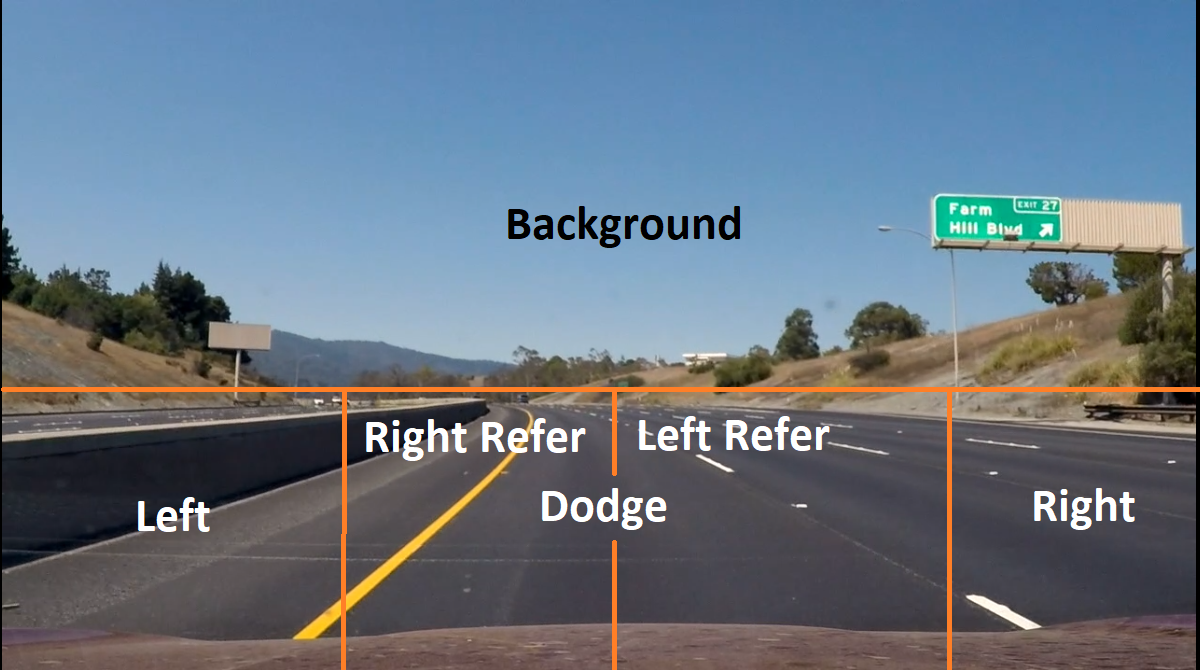
\includegraphics[width=.8\textwidth]{ch3/zones.png} % Include the image placeholder.png
		\caption{Phân vùng hình ảnh}
		\end{center}
		\end{figure}	

Sau khi nhận được tọa độ tâm của các vật thể, bằng việc xem xét vị trí tương ứng của từng tâm rơi vào vùng nào, thuật toán sẽ đưa ra quyết. Nhóm đề ra giải thuật như sau:

	\begin{enumerate}
		\item Kiểm tra có tồn tại vật thể trong vùng Dodge hay không? Nếu không có, tiếp tục đi thẳng và xét tiếp các tâm vật thể khác.
		\item Nếu tồn tại ít nhất một vật thể trong vùng Dodge, xác định xem tâm đó nằm trong phần nào của vùng Dodge (Left Refer hoặc Right Refer).
		\item Nếu vật thể nằm trong vùng Left Refer, ta kiểm tra xem bên vùng Left có tồn tại vật thể nào hay không. Nếu có, ta cho phương tiện chạy chậm lại, nếu không, ta cho phương tiện rẽ trái.
		\item Nếu vật thể nằm trong vùng Right Refer, ta kiểm tra xem vùng Right có tồn tại vật thể hay không. Nếu có, ta cho phương tiện chạy chậm lại, nếu không, ta cho phương tiện rẽ trái.	
	\end{enumerate}
Thuật toán được minh họa bằng sơ đồ giải thuật trong Hình.\ref{fig:flowchart}.

		\begin{figure}[h]
 		\label{fig:flowchart}
		\begin{center}
		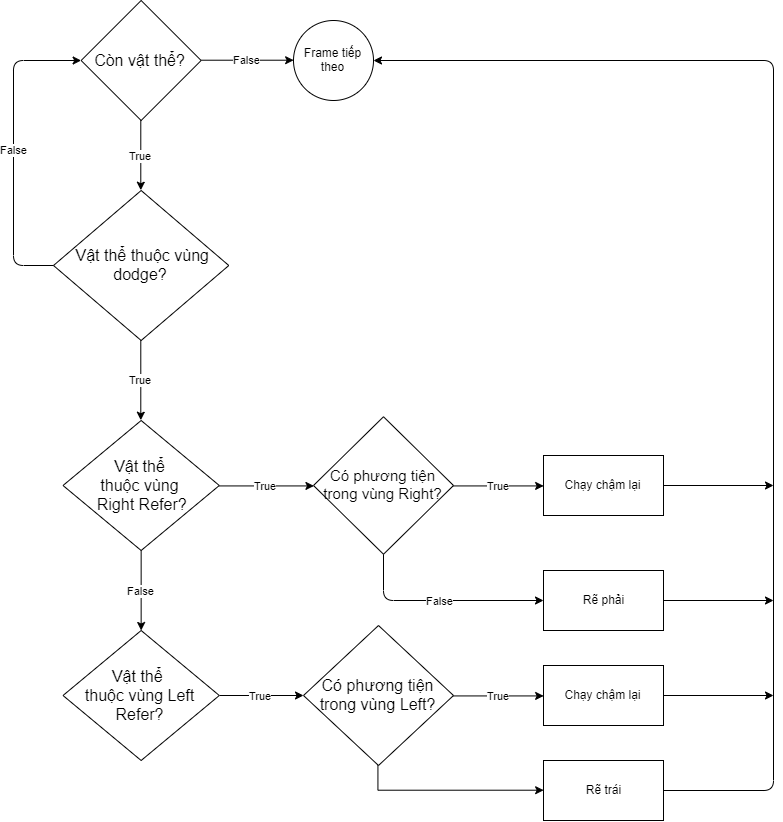
\includegraphics[width=.8\textwidth]{ch3/algo-flowchart.png} % Include the image placeholder.png
		\caption{Giải thuật ra quyết định}
		\end{center}
		\end{figure}	

\newpage